% Automaton corresponding to the formula phi = exists P. (Sing(P) and not P
% \subseteq X)

\documentclass{standalone}

\usepackage{pgf}
\usepackage{tikz}
\usepackage{amssymb}
\usetikzlibrary{arrows,automata}
\usepackage[latin1]{inputenc}
\begin{document}
%\begin{figure}
% \begin{center}
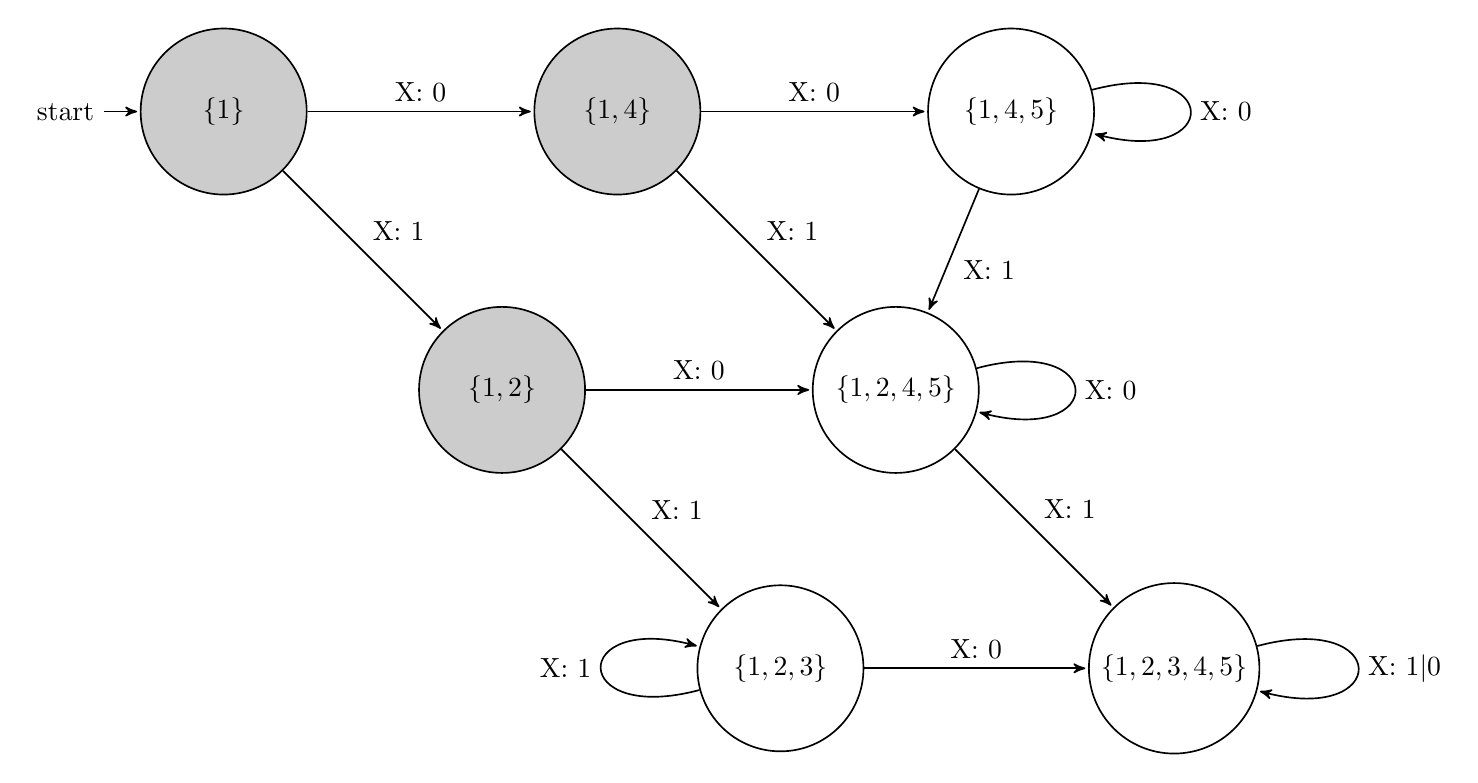
\begin{tikzpicture}[->,>=stealth',shorten >=1pt,auto,node distance=5cm,
                    semithick, transform shape]
  \tikzstyle{every state}=[fill=none,draw=black,text=black,minimum size=60pt]

  \node[initial,state,fill={rgb:black,1;white,4}] (A)                      
  {$\{1\}$}; \node[state,fill={rgb:black,1;white,4}]         (AD) [right of=A]  
  {$\{1, 4\}$};
  \node[state,fill={rgb:black,1;white,4}]         (AB) [below right of=A]  
  {$\{1, 2\}$}; \node[state]         (ADE) [right of=AD]       {$\{1, 4, 5\}$};
  \node[state]         (ABC) [below right of=AB] {$\{1, 2, 3\}$};
  \node[state]         (ABDE) [below right of=AD]    {$\{1, 2, 4, 5\}$}; 
  \node[state]         (ABCDE) [below right of=ABDE] {$\{1, 2, 3, 4, 5\}$};
  
  \path (A) edge                 node {X: 0}   (AD)
            edge                 node {X: 1}   (AB)
        (AD) edge                node {X: 0}   (ADE)
             edge                node {X: 1}   (ABDE)
        (AB) edge                node {X: 0}   (ABDE)
             edge                node {X: 1}   (ABC)
        (ADE) edge [loop right]  node {X: 0}   (ADE)
              edge               node {X: 1}   (ABDE)
        (ABC) edge               node {X: 0}   (ABCDE)
              edge [loop left]  node {X: 1}   (ABC)
        (ABDE) edge [loop right] node {X: 0}   (ABDE)
               edge              node {X: 1}   (ABCDE)
        (ABCDE) edge [loop right]node {X: 1\textbar 0}   (ABCDE);
\end{tikzpicture}
% \end{center}
% \caption{Automaton $\mathcal{A}_\phi$ corresponding to the formula $\phi =
% \exists P. (Sing(P) \wedge \neg P \subseteq X)$}
%\end{figure}
\end{document}